\documentclass[letterpaper]{article}
\usepackage{ms1report}
\usepackage[pdftex]{graphicx}
\usepackage{times}
\usepackage{helvet}
\usepackage{courier}
\usepackage[numbers]{natbib}
\pdfinfo{/Title (The Nature of Breath) /Author (Lauria Clarke)}

\title{The Nature of Breath: A Biomimetic Kinetic Sculpture That Breathes}
\author{Lauria Clarke\\ Parsons School of Design, The New School\\ New York, USA\\ clarl404@newschool.edu\\
\newline
\newline
}
\setcounter{secnumdepth}{0}

\begin{document} 
\maketitle

\begin{abstract}
the nature of breath is...
\end{abstract}

\keywords{Keywords}

%------------------------------
\section{Introduction}

% general introduction

Masahiro Mori's 1970 essay prvided the framework for describing the confusing relationship between artifically created human-like robots and, as Mori calls us, real human beings. \cite{mori} This framework of thought has gained significant traction over the last 50 plus years as developments in technology have made it possiblt to mimic the human body with increasing accuracy. This definition has also been critical in the field of computer science as we consinute ot refine mahcine learning techniques which steadily approach the capacities of the uhman brain. This framework describes the point at which an artificial automaton approaches a point of being eeriely similar to a human being, creating a feeling of discomfort via the uncertainty of whether it is "real".

For the lats fifty years this framework fo thought has been critical in describing technology's relationship with humanity. 

Over the last *** years however, the fields of biodesign and bioart have increasingly been asking similar questions not about tchnology and humanity, but technology and nature. In light of the increasing environmental pressures of human imposed climate change, these questions are becoming increasingly urgent. Technology is now being used t oreplicate and mimic natural systems. As Donna Haraway noted in her paper, we must thin kbeyond the human. \cite{haraway} The capacity of our technology has surpassed the instinctually introspective and can now mimic what is natural outside of ourselves. This is a critical development and harkens back to mode indigenous ways of thinking - moving and working with natural systems, rather than in opposition to. 

If our relationship with technology is extending beyond the human so to must our language. Mori's framework is distinctly human centric. How then do we apply this thinking to non-human natural world? Is Mori's valley merely a snaller depression within a much broader valley encompassing the whole of the natural world? Do humans deserve a place in that broader cintext? To frame this question more broadly, how do we, as human beings, distinguish between what is natural and what is atrificial? How is this distinction shifting as our techological capacity for the artifical increases at great cost to the natural world. 

Using the COVID-19 pandemic as lens and reference, this work attempts to lay a foundation for deeping inquiry into the above. While its focus is on a specifically human foram of respiration, respiration in broader context is omnipresent in living organisms, thus providing a jumping off point for larger scope of inquiry into the relationship between what it means to be alive and what it means to be natural. Something about being alive. \cite{zimmer}


\subsection{temporal relevance}
% the pandemic...the soundscape of the pandemic...
Teh COVID-19 pandemic has caused a sort of crystalization on many of the aforementioned optics, and has  

During the pandemic many people tried ot mkae ventilators at home. Segue...

\subsection{mechanical relevance}
% talk about the history of breathing apparatus and note that none mimic the human body
Mechanical ventilation has been around for a long time. Since it  seeks to provide "replacement of the respiratory muscles". \cite{ventilatorhistory} This results in apparati that resembly the respiratory system only in the sens that they cause a regutaled chnage in pressure, but have no need for recreating htep rocess by which breaht sounds are actually created. Simialrly, the cield of biomemtic robotics has little use for such inquiry - respiration is not necessary for an electronic humanoid and it is much easier to produce vocal noises in a digital manner. 

Two notable works in the field of kinetic sculpture provide reference, Mawa Denkye's lauching machine and another guy's breath machine thing. These two pieces provoke thought about breath, but still use simple bellow bases mechanisms to produce airflow. %\cite{deynke} \cite{otherguy}

% need to figure out how to combine the two naturally
\section{prior work}

mawa deynke 

breath thing from bitforms

homemade ventilators


\section{implementation}

broken down into two steps; thinking and making

\subsection{system breakdown}

the respiratory system is complex, so I made is simpler

\subsubsection{actuation}

how air is moved through the respiratory system

\subsubsection{storage}

how air is stored in the respiraatory system

\subsubsection{modulation}

how the sound of breath is created

\subsection{making}

So far a few different protptypes ahve been attempted. Focusing on the two main areas of inquiry, there have been auditory prototypes, exploring the effect os disembodied breath noises, as well as machnical prototypes, exploring ways to achieve a physiologically accurate breahting mechanism. 

\subsubsection{auditory prototypes}

bucket experiement

p5 thing

\subsubsection{physical prototypes}

trachea

diaphragm

lever adjustment

\subsubsection{final prototypes}

the final result was a thing that nearly works and combines many of the elements from above

\section{further work}

there's always more to do...

the boris vian reference 


\section{conclusion}

talk about the big distinction of artificial and natural

why it's important to think about this in the context of humanity's relationship with the natural world


%\begin{figure}[h]
%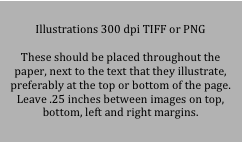
\includegraphics[width=3.31in]{figure.png}
%\caption{This is an example of figure caption. Note that all figures, and tables are to be referenced in the text. \copyright Respect Copyright.}
%\end{figure}
%
%\begin{figure*}
%
\includegraphics[width=\textwidth]{two-column-figure.png}
%\caption{Example of a double-column figure with caption. \copyright Respect Copyright.}
%\end{figure*}


\bibliographystyle{plain}
\bibliography{ms1report}

\section{Bibliography}
%The difference between a reference list and a bibliography is that in your references, you list all the sources you directly referred to in the body of your writing in numerical order, whereas a bibliography includes an alphabetical listing of all those authors and sources that you have consulted while writing your essay. Use the same format as for the references otherwise. Those using Latex will follow the usual cite command format.

\section{Author Biography}
Lauria Clarke is an engineer and artist living in New York. She completed an MS in Computer Engineering at Northeastern University in 2017 and is currently persuing an MFA in Design and Technology at The Parsons School of Design. She specializes in digital hardware design and kinetic sculpture and is always curious to learn more about humanity's relationship with the natural world.

% aspires to be a chocolate fish fisherman for Ben and Jerry's.


\end{document}
